%&latex
\documentclass[a4paper]{article}

\frenchspacing

\usepackage[cp1250]{inputenc}
\usepackage[czech]{babel}

\usepackage{a4wide}
\usepackage{amsmath, amsthm, amssymb, amsfonts}
\usepackage[mathcal]{eucal}
\usepackage{graphicx}
\usepackage{url}
\usepackage{color}
\usepackage{wrapfig}
\usepackage{capt-of}
\usepackage{float}
\usepackage{ifthen}
\usepackage{subfig}
\usepackage[normalem]{ulem}


% sirka a vyska textu nastavena jako papir, vsechny okraje vynulovany a pridano 20pt na kazdou stranu
% horizontalni rozmery
\setlength{\textwidth}{\paperwidth}
\addtolength{\textwidth}{-40pt}
\addtolength{\hoffset}{-1in}
\addtolength{\hoffset}{20pt}
\setlength{\oddsidemargin}{0in}
\setlength{\marginparsep}{0in}
% vertikalni rozmery
\setlength{\textheight}{\paperheight}
\addtolength{\textheight}{-60pt}
\addtolength{\voffset}{-1in}
\addtolength{\voffset}{20pt}
\setlength{\topmargin}{0in}
\setlength{\headheight}{0in}
\setlength{\headsep}{0in}


%Obrazek na miste
%pouziti
%%\obrazeknahore{adresa}{popisek}{label}
\long\def\obrazeknahore#1#2#3 {

\begin{figure}[t]
    \centering
    \includegraphics[width=0.8\textwidth]{#1}
    
    \caption{#2}
    \label{#3}
    
\end{figure}

}


%==========================================
%PEKELNA MAKRA NA ZAROVNANI OBRAZKU DOPRAVA

\makeatletter


%tohle je makro, ktere mi dovoluje obtekani i u kratkych environmentu
%ABSOLUTNE nechapu, jak to funguje, ale funguje to
%viz http://tex.stackexchange.com/questions/26078/ 
\def\odrovnej{\@@par
\ifnum\@@parshape=\z@ \let\WF@pspars\@empty \fi % reset `parshape'
\global\advance\c@WF@wrappedlines-\prevgraf \prevgraf\z@
\ifnum\c@WF@wrappedlines<\tw@ \WF@finale \fi}

\makeatother



%---
%makro, co da obrazek doprava a ostatni text ho obteka
%(bez toho predchazejiciho makra to ale poradne nebeha)
%pouziti:
%\obrazekvpravo{adresa}{popisek}{label}{procento sirky}
\long\def\obrazekvpravo#1#2#3#4{

\setlength\intextsep{-20pt}

    \begin{wrapfigure}{r}{#4\textwidth}
      \begin{center}
          \vspace{-10pt}
          
        \includegraphics[width=#4\textwidth]{#1}
        \vspace{-10pt}
        
      \end{center}
      
      \caption{#2}
      \label{#3}
      
      
    \end{wrapfigure}

\setlength\intextsep{0pt}

    
}




%---
%makro pro pripady, kdy wrapfigure neco mrsi
%je to docela pekelne
%je nutne mu dat jak text vpravo, tak text vlevo
%a nevim, jestli bude 100% fungovat, ale doufam, ze jo

%pouziti:
%\obrazekvpravominipage{adresa}{popisek}{label}{procento sirky}{1 - procento sirky}{text vlevo}
\long\def\obrazekvpravominipage#1#2#3#4#5#6{

\noindent\begin{minipage}{#5\linewidth}
\vspace{0pt}
#6
\end{minipage}
\hspace{0.5cm}
\noindent\begin{minipage}{#4\linewidth}
\vspace{0pt}
\centering
\includegraphics[width=0.9\textwidth]{#1}
\captionof{figure}{#2}
\label{#3}
\end{minipage}

}

%KONEC PEKELNYCH MAKER
%=====================

\def\lebka{
\includegraphics[width=3mm]{../common/lebka}}

% makra pro poznamku u vyrokove a predikatove logiky
\def\vl{ -- ve v�rokov� logice}
\def\pl{ -- v predik�tov� logice}


%Vacsina prostredi je dvojjazicne. V pripade, ze znenie napr pozorovania je pisane po slovensky, malo by byt po slovensky aj oznacenie.

\def\ifis#1#2{\ifthenelse{\equal{#1}{0}}{}{#2}}

%\newenvironment{e}[3]{\pagebreak[2]\noindent\textbf{\ifis{#2}{$\bigstar$}#1}\ifis{#3}{\emph{~(#3)}}\par\noindent\leftskip 10pt }{\odrovnej\par\bigskip}
\newenvironment{e}[3]{\pagebreak[2]\noindent\textbf{\ifis{#2}{\lebka~}#1}\ifis{#3}{\emph{~(#3)}}\ifis{#2}{~\lebka}\par\noindent\leftskip 10pt }{\odrovnej\par\bigskip}


%obecne prostredie, ktore ma vyuzitie pri specialnych odstavcoch ako (uloha, algoritmus...) aby nevzniklo dalsich x prostredi
\newenvironment{obecne}[1]{\pagebreak[2]\noindent\textbf{#1}\par\noindent\leftskip 10pt}{\odrovnej\par\bigskip}

\newenvironment{report}{\pagebreak[2]\noindent\textbf{Report}\em\par\noindent\leftskip 10pt}{\par\bigskip}

%\newenvironment{reportN}[1]{\pagebreak[2]\noindent\textbf{Report~}\emph{(#1)}\emph\par\noindent\leftskip 10pt}{\odrovnej\par\bigskip}
\newenvironment{reportN}[1]{\pagebreak[2]\noindent\textbf{Report~}\emph{(#1)}\em\par\noindent\leftskip 10pt}{\odrovnej\par\bigskip}

\newenvironment{penumerate}{
\begin{enumerate}
  \setlength{\itemsep}{1pt}
  \setlength{\parskip}{0pt}
  \setlength{\parsep}{0pt}
  %\setlength{\topsep}{200pt}
  \setlength{\partopsep}{200pt}
}{\end{enumerate}}

\def\pismenka{\numberedlistdepth=2} %pouzit, ked clovek chce opismenkovany zoznam...

\newenvironment{pitemize}{
\begin{itemize}
  \setlength{\itemsep}{1pt}
  \setlength{\parskip}{0pt}
  \setlength{\parsep}{0pt}
}{\end{itemize}}

\definecolor{gris}{gray}{0.95}
\newcommand{\ramcek}[2]{\begin{center}\fcolorbox{white}{gris}{\parbox{#1}{#2}}\end{center}\par}


\title{\LARGE U�ebn� texty k st�tn� bakal��sk� zkou�ce \\ Matematika \\ Algebra}

\begin{document}

\maketitle

\newpage
\setcounter{section}{7}
\setcounter{page}{58}
%&latex
\def\Real{\mathbb{R}}
\def\Whole{\mathbb{Z}}
\def\Complex{\mathbb{C}}
\def\Rational{\mathbb{Q}}
\def\Nat{\mathbb{N}}
\def\ifandonlyif{\ \Leftrightarrow\ }
\def\implies{\ \Rightarrow\ }
\def\lmod{\mathrm{lmod}}
\def\rmod{\mathrm{rmod}}
\def\ker{\mathrm{ker}}
\def\id{\mathbf{id}}
\def\NSD{\mathbf{NSD}}
\def\deg{\mathrm{deg}\ }
\def\st{\mathrm{st}\ }

\section{Algebra}

\begin{e}{Po�adavky}{0}{0}
\begin{pitemize}
    \item Grupa, okruh, t�leso -- definice a p��klady
    \item Podgrupa, norm�ln� podgrupa, faktorgrupa, ide�l
    \item Homomorfismy grup 
    \item D�litelnost a ireducibiln� rozklady polynom� 
    \item Rozklady polynom� na ko�enov� �initele pro polynom s re�ln�mi, racion�ln�mi, komplexn�mi koeficienty. 
    \item N�sobnost ko�en� a jejich souvislost s derivacemi mnoho�lenu
\end{pitemize}
\end{e}


\subsection{Grupa, okruh, t�leso -- definice a p��klady}

\begin{e}{Definice}{0}{algebra}
Pro mno�inu $A$ je zobrazen� $\alpha : A^n \to A$, kde $ n \in \{0,1, ...\}$ \emph{n-�rn� operace} ($n$ je \emph{arita}). Jsou-li $\alpha_i, i \in I$ operace arity $\Omega_i$ na $A$, pak $(A, \alpha_i|i\in I )$ je \emph{algebra}.
\end{e}

\begin{e}{Definice}{0}{grupoid, monoid}
Algebra s 1 bin�rn� operac� je \emph{grupoid}. V n�m m��e b�t $e\in G: e\cdot g = g\cdot e = g\ \forall g\in G$ \emph{neutr�ln� prvek}. 

Algebra s jednou asociativn� \emph{je mo�no p�ez�vorkovat}  bin�rn� operac� a neutr�ln�m prvkem vzhledem k n� je \emph{monoid}. Nech� je d�n monoid s neutr�ln�m prvkem $(M, \cdot,e)$ a n�jak�m prvek $m\in M$. Potom �ekneme, �e prvek $m^{-1}\in M$ je \emph{inverzn�} k prvku $m$, pokud $m\cdot m^{-1} = m^{-1}\cdot m = e$. Prvek je \emph{invertibiln�}, pokud m� n�jak� inverzn� prvek.
\end{e}

\begin{e}{Pozn�mka}{0}{0}
Ka�d� grupoid obsahuje nejv�� 1 neutr�ln� prvek. V libovoln�m monoidu plat�, �e pokud $(a\cdot b = e)\ \&\ (b\cdot c = e)$, pak $a = c$ (tj. inverzn� prvek zleva a zprava mus� b�t ten sam�). Ka�d� inverzn� prvek je s�m invertibiln�.
\end{e}

\begin{e}{Definice}{0}{grupa}
Algebra $(G,\cdot,^{-1},e)$ je \emph{grupa}, pokud je $(G,\cdot,e)$ monoid a $^{-1}$ je operace inv. prvku (tedy un�rn� operace, kter� ka�d�mu prvku p�i�ad� prvek k n�mu inverzn�).
Grupa $G$ je \emph{komutativn� (abelovsk�)}, pokud je operace \uv{$\cdot$} komutativn�.
\end{e}

\begin{e}{P��klady}{0}{0}
P��klady grup:
\begin{pitemize}
    \item Mno�ina $\Real$ s operac� s��t�n�, inverzn�m prvkem $-x$ a neutr�ln�m prvkem $0$
    \item Mno�ina $\Real_{+}$ (kladn�ch re�ln�ch ��sel, tedy bez nuly, proto�e k t� bychom inverzn� prvek nena�li) s operac� n�soben�, inverzn�m prvkem $x^{-1}$ a neutr�ln�m prvkem $1$
    \item Mno�ina $\Whole_n=\{0,\dots,n-1\}$ pro $n$ libovoln� p�irozen� ��slo; s operac� s��t�n� modulo $n$, inverzn�m prvkem $(-x)$ modulo $n$ a neutr�ln�m prvkem $0$
    \item Mno�ina polynom� stupn� $\leq n$ se s��t�n�m, opa�n�m polynomem (s opa�n�mi koeficienty) a neutr�ln�m prvkem $0$
    \item Mno�ina v�ech permutac� prvk� $(1,\dots,n)$ s operac� skl�d�n� permutac�, opa�nou permutac� (takovou, �e jej� slo�en� s p�vodn� d�v� identitu) a neutr�ln�m prvkem $\id$ (na rozd�l od v�ech p�edchoz�ch pro permutace d�lky v�t�� ne� 3 nen� abelovsk�)
    \item Mno�ina regul�rn�ch matic $n\times n$ s operac� maticov�ho n�soben�, inverzn�mi maticemi a jednotkovou matic� (takt� nen� obecn� abelovsk�)
\end{pitemize}
\end{e}


\begin{e}{Definice}{0}{okruh}
Nech� $(R,+,\cdot,-,0,1)$ je algebra takov�, �e $(R,+,-,0)$ tvo�� komutativn� grupu, $(R,\cdot,1)$ je monoid a plat� $a(b+c)=ab+ac$ a $(a+b)c=ac+bc\ \forall a,b,c\in R$ (tedy distributivita n�soben� vzhledem k s��t�n�\footnote{�emli�ka p�e ve skriptech s��t�n� v��i n�soben�, ale v literatu�e se to p�e v�t�inou obr�cen� (asi to ale bude to sam�)}). Pak je $(R,+,\cdot,-,0,1)$ \emph{okruh}.\footnote{"--" je v n�m st�le un�rn� operace}
\end{e}

\begin{e}{P��klady}{0}{0}
P��klady okruh�:
\begin{pitemize}
    \item Mno�ina $\Whole$ s operacemi s��t�n� a n�soben�, inverzem v��i s��t�n� -- un�rn�m minus a neutr�ln�mi prvky $0$ a $1$.
    \item Mno�ina v�ech line�rn�ch zobrazen� na $\Real^n$ s operacemi s��t�n� a skl�d�n�, \uv{opa�n�m} zobrazen�m (kde $(-f)(x)=-(f(x))$), nulov�m zobrazen�m a identitou (pro obecn� zobrazen� toto nefunguje, neplat� distributivita)
\end{pitemize}
\end{e}


\begin{e}{Pozn�mka}{0}{Vlastnosti okruh�}
V okruhu $(R,+,\cdot,-,0,1)$ pro ka�d� 2 prvky $a,b\in R$ plat�: 
\begin{penumerate}
    \item $0\cdot a = a\cdot 0 = 0$
    \item $(-a)\cdot b = a\cdot(-b)=-(a\cdot b)$
    \item $(-a)\cdot(-b)=a\cdot b$
    \item $|R|>1 \ifandonlyif 0 \neq 1$
\end{penumerate}
\end{e} 

\begin{e}{Definice}{0}{t�leso}
\emph{T�leso} je okruh $(F,+,-,\cdot,0,1)$, pro kter� nav�c plat�, �e pro ka�d� $x\in F$ krom� nuly existuje $y\in F$ takov�, �e $x\cdot y = y\cdot x = 1$, tj. pro v�echny prvky krom� nuly existuje inverzn� prvek v��i operaci \uv{$\cdot$} -- \uv{$x^{-1}$}. Nav�c v $F$ mus� platit, �e $0\neq 1$ (vylou�en� trivi�ln�ch okruh�).  

\emph{Komutativn� t�leso} je takov� t�leso, ve kter�m je operace \uv{$\cdot$} komutativn�.
\end{e}

\begin{e}{P��klady}{0}{0}
P��klady t�les:
\begin{pitemize}
    \item T�lesa $\Complex$ a $\Real$, oproti tomu $\mathbb{Z}$ nebo $\mathbb{N}$ nejsou t�lesa - nemaj� inverzn� prvek k n�soben�
    \item Racion�ln� ��sla $\Rational = \{ \frac{a}{b}\ | a,b\in\Whole, b\neq 0\}$
    \item $\Whole_{p^{n}}=\{0,\dots,p^n-1\}$, kde $p$ je prvo��slo a $n$ p�irozen� ��slo -- tzv. \emph{Gallois field}, pro dan� $p$ a $n$ existuje v�dy a� na isomorfismus (p�ejmenov�n� prvk�) jen jedno.
- \emph{ka�d� kon. t�leso m� $p^n$ prvk� (KAM TO PATRI???)}
    \item $(\Whole_p,+,-,\cdot,0,1)$ je komutativn� t�leso charakteristiky p, ted obor integrity
\end{pitemize}
V�echna uveden� t�lesa jsou komutativn�.
\begin{center}
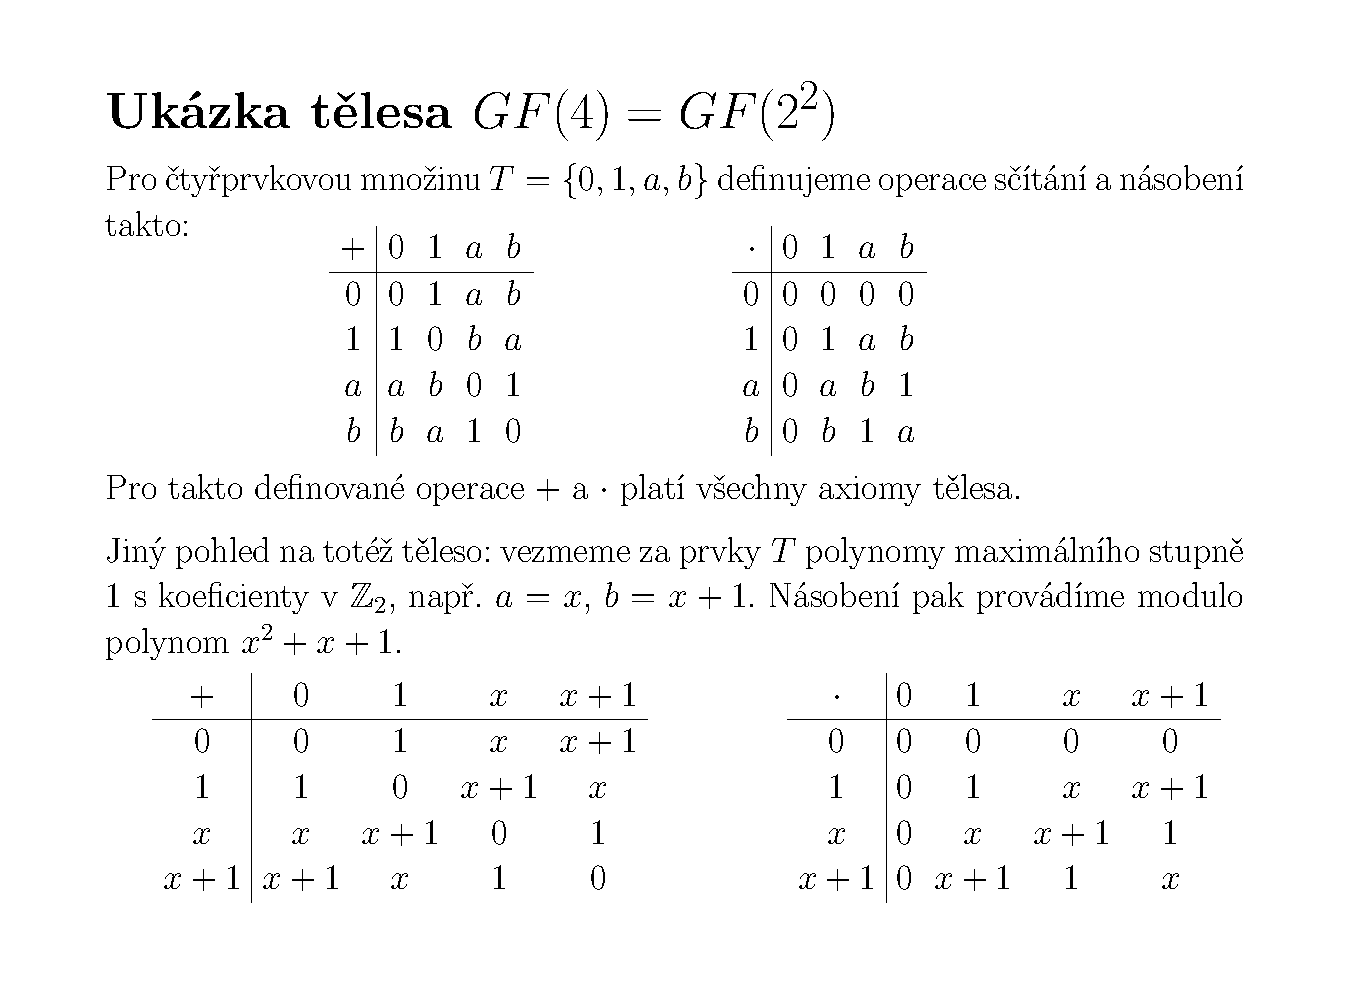
\includegraphics[scale=0.5]{matematika/obrazky/teleso_GF4}
\end{center}
\end{e}
\begin{e}{V�ta}{1}{Wedderburnova v�ta}
V�echna kone�n� t�lesa jsou komutativn�.
\end{e} 
\begin{reportN}{IOI 10.2.2011} Napi�te definici t�lesa. Rozhodnete, zda existuje konene t�leso ��du $k$ pro hodnoty $k$ z mno�iny $\{2,3,4,6,7,8\}$. P�ipome�me, �e ��d t�lesa je po�et jeho prvk�. Zvolte si nyn� libovoln� komutativni
t�leso T ��du 5,
\\
a) Popi�te pomoc� tabulky, jak jsou v tomto t�lese definov�ny operace s��t�n� a n�soben� 
\\b)Vysv�tlete, co znamen�, �e t�leso T je komutativni.
\\c) Udejte p��klad nekomutativn�ho t�lesa ��du 9 nebo zd�vodn�te, pro� takov� t�leso neexistuje
\end{reportN}
\begin{center}
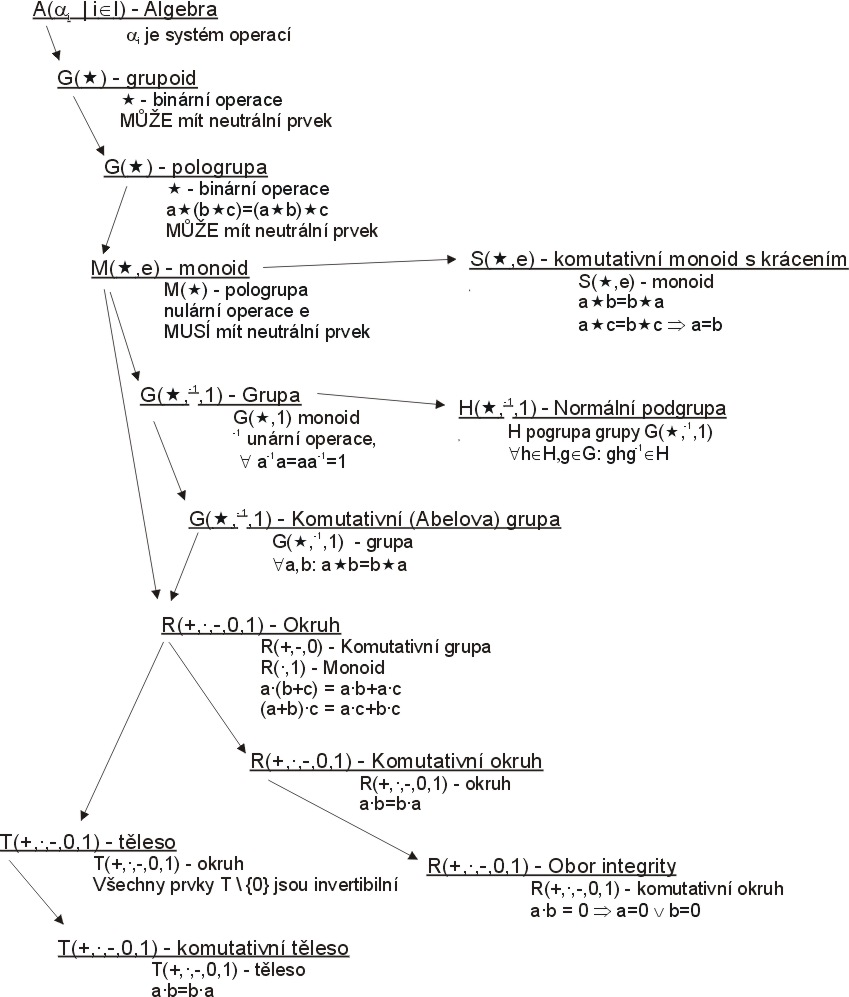
\includegraphics[scale=0.5]{matematika/obrazky/algebra_struktury}
\\prost� d�di�nost jako z C++ 
\end{center}

\subsection{Podgrupa, norm�ln� podgrupa, faktorgrupa, ide�l}

\begin{e}{Definice}{0}{podalgebra}
Mno�ina $B$ je \emph{uzav�en�} na operaci $\alpha$, kdy� $\forall b_1,\dots b_n \in B$ plat� $\alpha(b_1, ... b_n) \in B$. Pro algebru $(A, \alpha_i|i\in I)$ je mno�ina $B\subseteq A$ spolu s operacemi $\alpha_i$ \emph{podalgebra} $A$, je-li mno�ina $B$ uzav�en� na operaci $\alpha_i\ \forall i\in I$.
\end{e}

\begin{e}{Definice}{0}{podgrupa}
Podalgebra grupy je \emph{podgrupa} (tj. jde o podmno�inu p�v. mno�iny prvk�, uzav�enou na \uv{$\cdot$} a \uv{$^{-1}$}, spolu s p�vodn�mi operacemi). Podgrupa $H$ grupy $G$ je \emph{norm�ln�}, pokud pro ka�d� $g \in G$ (z p�vodn� mno�iny!) a pro ka�d� $h \in H$ plat�, �e $g^{-1}\cdot h\cdot g \in H$ (n�kdy se p�e zkr�cen� $G^{-1}HG\subseteq H$).
\end{e}

\begin{e}{Pozn�mka}{0}{Vlastnosti podgrup}
Pr�nik podgrup $G\cap H$ je op�t podgrupa. To ur�it� neplat� o sjednocen� $G\cup H$ (to je podgrupou jen pokud je $G\subset H$ nebo $H\subset G$). Ka�d� podmno�ina grupy m� n�jakou nejmen�� podgrupu, kter� ji obsahuje -- to je \emph{podgrupa generovan�} touto \emph{mno�inou}. Podgrupa (i grupa) generovan� jedn�m prvkem se naz�v� \emph{cyklick�}. Ka�d� podgrupa cyklick� grupy je tak� cyklick�. 

Podgrupy ka�d� grupy spole�n� s pr�nikem jako infimem a podgrupou generovanou sjednocen�m jako supremem tvo�� �pln� svaz (algebru se dv�ma operacemi se speci�ln�mi vlastnostmi, supremem a infimem, definovan�mi pro v�echny jej� podmno�iny). �pln� svaz se stejn�mi operacemi tvo�� tak� norm�ln� podgrupy (jde o podsvaz prvn�ho).
\end{e}
\begin{e}{Pozn�mka}{0}{Vlastnosti cyklick�ch podgrup}
Ka�d� cyklick� grupa G je komutativn� (Abelova).
\proof
Proto�e $x,y\in G$ pak $x,y=a^m.a^n=a^{m+n}=a^{n+m}=y.x$
\end{e}

\begin{e}{P��klady}{0}{0}
P��klady podgrup:
\begin{pitemize}
    \item grupa re�ln�ch ��sel uzav�en� na s��t�n� nen� cyklick�
    \item $G$ a $\{e\}$ jsou v�dy norm�ln� podgrupy grupy $(G,\cdot,^{-1},e)$. 
    \item Mno�ina $Z(G)=\{z\in G|gz = zg\ \forall g\in G\}$ je norm�ln� podgrupou $G$ (\uv{\emph{centrum grupy}}).
    \item $\Whole_8$ m� dv� netrivi�ln� podgrupy -- $\{0,4\}$ a $\{0,2,4,6\}$ (je sama cyklick�, tak�e ob� jsou cyklick�), plus samoz�ejm� trivi�ln� $\Whole_8$ a $\{0\}$.
    \item grupa $(\Whole_8^*,\cdot,1)$ nen� cyklick�\footnote{$\Whole_8^*$
    je $\Whole_8$ obsahuj�c� invertibiln� prvky ($[0]_8$ ne)}, skl�d� se z 4 prvk�: $\Whole_8^*=\{1,3,5,7\}$ a $3^2=5^2=7^2=1^2 =1$ 
\end{pitemize}
\end{e}

\begin{e}{Definice}{0}{0}
Pro grupu $G$ a jej� podgrupu $H$ se relace $\rmod_H$ definuje p�edpisem  $a,b\in G:(a,b)\in\rmod_H\equiv ab^{-1}\in H$. Symetricky se definuje relace $\lmod_H$ ($(a,b)\in\lmod_H\equiv a^{-1}b\in H$). Tyto relace jsou ekvivalence. \emph{Index podgrupy v grup�} je $[G:H]=|G/\rmod_H|=|G/\lmod_H|$ (po�et t��d ekvivalence podle $\rmod_H$ nebo $\lmod_H$).
\\\\\emph{��d} G (po�et jeho prvk� grupy) se zna�� $|G|$.

\begin{center}
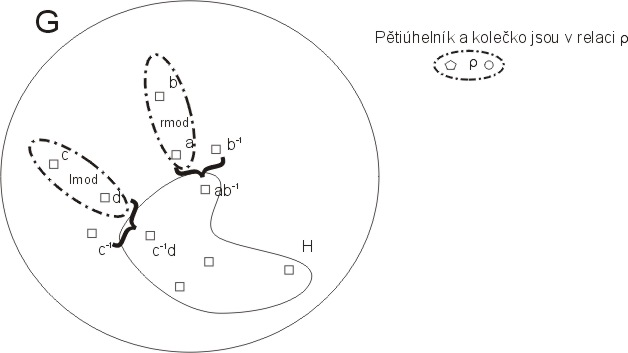
\includegraphics[scale=0.6]{matematika/obrazky/lmod_rmod}
\end{center}
\end{e}

\begin{e}{V�ta}{1}{Lagrangeova}
Pro grupu $G$ a jej� podgrupu $H$ plat�: $|G|=[G:H]\cdot|H|$. Z toho plyne, �e velikost podgrupy d�l� velikost kone�n� grupy.



\begin{e}{Idea d�kazu}{0}{0}

Nejd��ve je nutno dok�zat, �e lmod $H$ a rmod $H$ jsou ekvivalence (jsou reflexivn�, symetrick�, tranzitivn�) - vypl�v� z vlastnost� $^{-1}$. 

Potom je nutno uk�zat, �e $[a]_{\rmod H}$, tj. t��da ekvivalence ur�ena podle prvku $a$, je tot�, co $Ha$ (tj. prvky $H$ pron�sobeny $a$ \uv{zprava}) -- m�rn� pracn�.

Potom se uk�e, �e vyn�soben� zprava je bijekce, tj. $H\rightarrow [a]_{\rmod H}$ je bijekce, tj. $|H|=\left|[a]_{\rmod H}\right| \forall a \in G$, tj. t��dy ekvivalence jsou v�echny stejn� velk�, z �eho� u� v�ta plyne.

\end{e}

\begin{center}
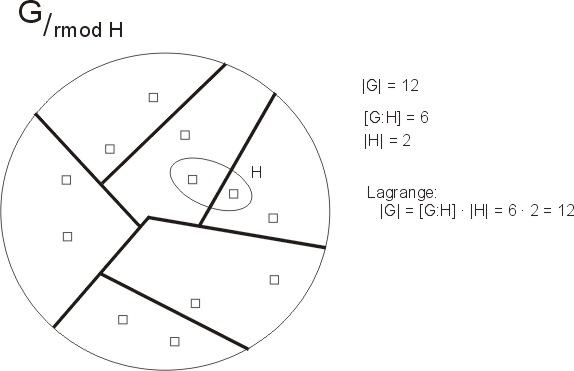
\includegraphics[scale=0.6]{matematika/obrazky/lagrange_algebra}
\\Index podgrupy $H$ v grup� $G$ ($[G:H]$) je prost� po�et t��d ekvivalence relace $\rmod H$. D�le ��d grupy $|G|$ a uk�zka Lagrangeovy v�ty v praxi. 
\end{center}

\end{e}

\begin{e}{ Definice}{0}{0}
$H,K$ jsou podgrupy $G(\cdot,^{-1},1),\ g\in G:\ \emph{HK}= \{h.k |\
h\in H\,k\in K\}, \ \emph{gH}= \{g\}H,\ \emph{Hg}= H\{g\}$ 

(tato definice byla pou�ita v minul�m d�kazu :-))

\begin{center}
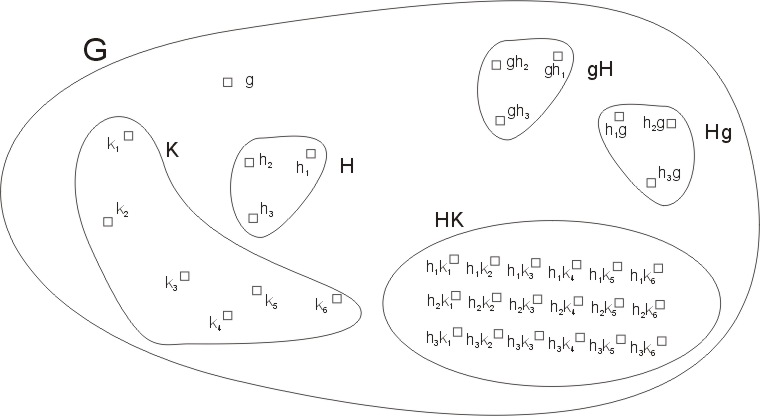
\includegraphics[scale=0.5]{matematika/obrazky/nasobeni_mnozin}
\end{center}
\end{e}

\begin{e}{Definice}{0}{faktorgrupa}
Pro grupu $(G,\cdot,^{-1},e)$ a n�jakou jej� norm�ln� podgrupu $N$ je \emph{faktorgrupa} $G/N=\{gN|g\in G\}$ kde $gN=\{g.n|n\in N\}$  ($gN$ se naz�v� lev� \emph{rozkladov� t��da}). $gN = [g]_{\lmod N}$.
\\\\
Tedy faktorgrupa je mno�ina v�ech lev�ch rozkladov�ch t��d podle n�jak� norm�ln� podgrupy. Faktorgrupa cyklick� nebo abelovsk� grupy je tak� cyklick�, resp. abelovsk�.
\end{e}

\begin{e}{P��klady}{0}{0}
P��klady faktorgrup:
\begin{pitemize}
    \item Pro grupu cel�ch ��sel $\Whole$ a jej� norm�ln� podgrupu sud�ch cel�ch ��sel $2\Whole$ je $\Whole/2\Whole$ faktorgrupou, isomorfn� s grupou $\{0,1\}$. Podobn� to plat� pro libovoln� $n\Whole$, kde $n$ je p�irozen�.
    \item $\Real/\Whole$ je faktorgrupa grupy $\Real$ (rozkladov� t��dy jsou tvaru $a + \Whole$, kde $a$ je re�ln� ��slo v intervalu $\langle 0,1)$.
    \item Faktorov� grupa $\Whole_4/\{0,2\}$ je isomorfn� se $\Whole_2$.     \item grupa $G = \{0, 1, 2, 3, 4, 5\}$ s operac� + s mod 6 a jej� norm�ln� podgrupu $N = \{0, 3\}$ pak faktorgrupa je definov�na jako $G/N = \{ gN | g\in G \} = \{ g\{0, 3\} | g\in\{0, 1, 2, 3, 4, 5\} \} = \newline
\{ 0\{0, 3\}, 1\{0, 3\}, 2\{0, 3\}, 3\{0, 3\}, 4\{0, 3\}, 5\{0, 3\} \} = \newline
\{ \{(0+0)\mod 6, (0+3) \mod 6\}, \{(1+0) \mod 6, (1+3) \mod 6\},
\newline        
        \{(2+0) \mod 6, (2+3) \mod 6\}, \{(3+0) \mod 6, (3+3) \mod 6\},
\newline        
        \{(4+0) \mod 6, (4+3) \mod 6\}, \{(5+0) \mod 6, (5+3) \mod 6\} \}=
\newline
    \{ \{0, 3\}, \{1, 4\}, \{2, 5\}, \{3, 0\}, \{4, 1\}, \{5, 2\} \} =
\newline    
    \{ \{0, 3\}, \{1, 4\}, \{2, 5\}, \{0, 3\}, \{1, 4\}, \{2, 5\} \} =
\newline    
    \{ \{0, 3\}, \{1, 4\}, \{2, 5\} \} $
\begin{center}
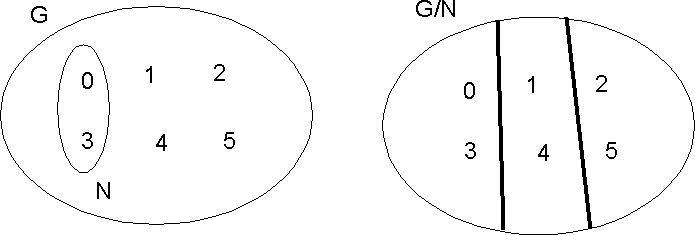
\includegraphics[width=0.8\textwidth]{matematika/obrazky/faktorgrupy}
\end{center}
\item $\Whole/6\Whole$
\begin{center}
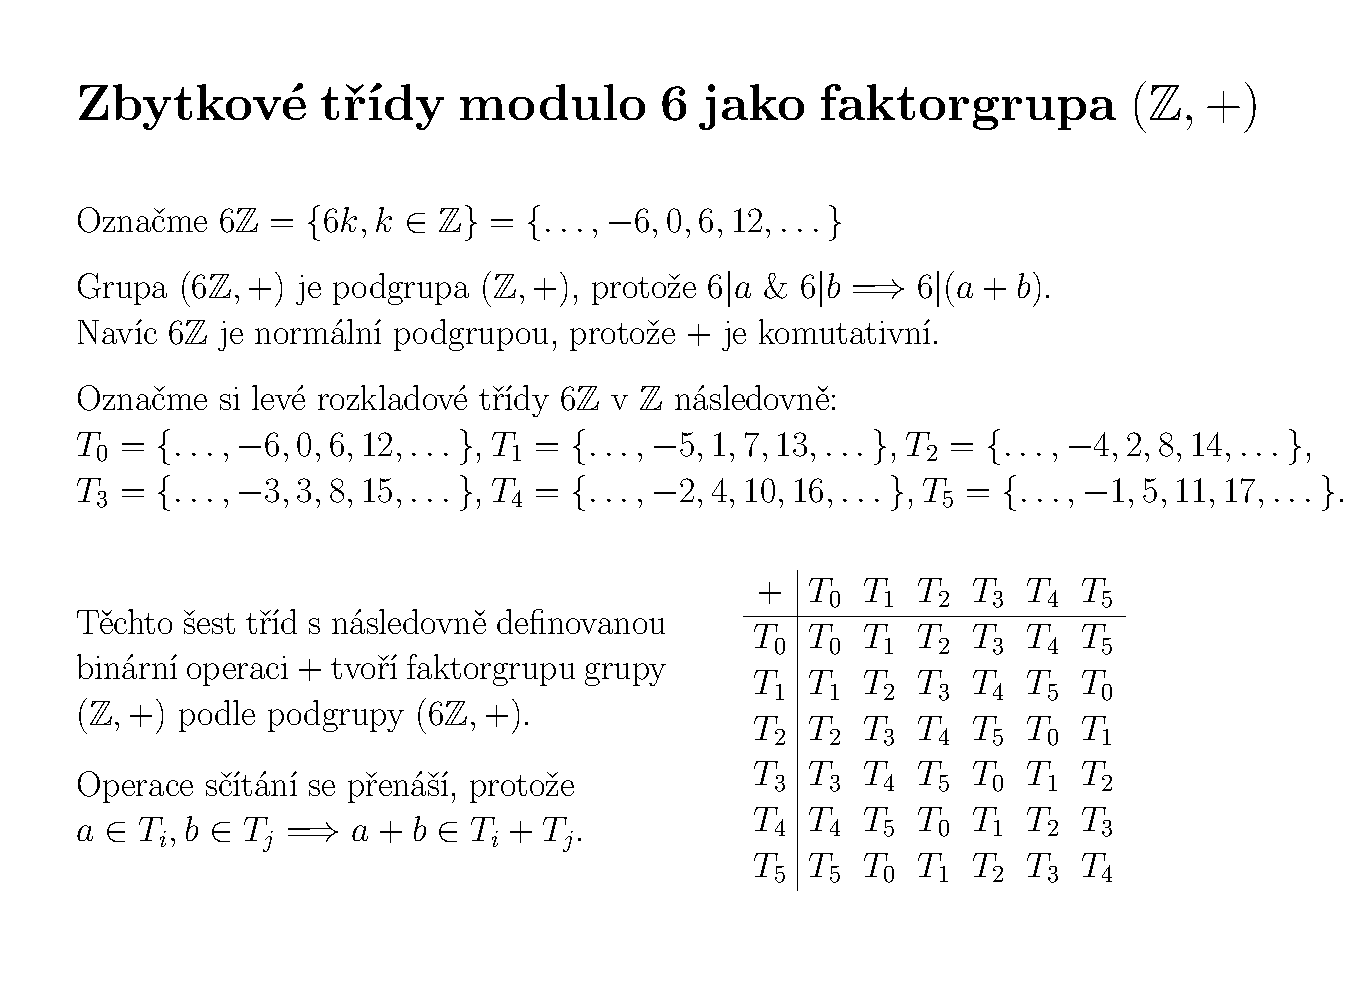
\includegraphics[width=0.7\textwidth]{matematika/obrazky/faktorgrupa}
\end{center}
\end{pitemize}
\end{e}

\begin{e}{Definice}{0}{kongruence}
Obecn� v algebr�ch je \emph{ relace $\rho$ slu�iteln� s operac� $\alpha$} arity $n$, pokud $a_1,\dots a_n, b_1,\dots b_n : (a_i,b_i)\in\rho\ \forall i$ 
\\
\noindent implikuje $(\alpha(a_1, \dots a_n), \alpha(b_1, \dots b_n))\in\rho$. \emph{Kongruence} je ka�d� ekvivalence slu�iteln� se v�emi operacemi algebry.
\end{e}

\begin{center}
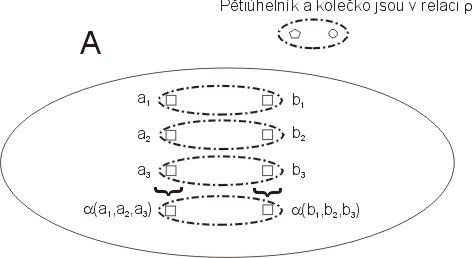
\includegraphics[scale=0.6]{matematika/obrazky/relace_slucitelna_s_operaci}
\\Relace $\rho$ slu�iteln� s operac� $\alpha$, �esky �e�eno, m�m-li n-�rn� operaci, tak pro ka�d� dv� n-tice pro kter� plat�, �e odpov�daj�c� si slo�ky n-tice jsou v relaci, tak v�sledky operace mus� b�t tak� v relaci. 
\end{center}

\begin{e}{Pozn�mka}{0}{0}
Faktorgrupa je vlastn� grupa, v n� jsou jednotliv� prvky t��dy ekvivalence na p�vodn� grup� podle n�jak� kongruence (lev� rozkladov� t��dy tvo�� kongruence).
\end{e}

\begin{e}{Definice}{0}{ide�l}
Nech� $(R,+,\cdot,-,0,1)$ je okruh a $I\subseteq R$. Pak $I$ je \emph{prav�(lev�) ide�l}, pokud
    $I$ podgrupa $(R,+,-,0)$ (je i norm�ln�, proto�e $R$ je z def. okruhu komutativn�) a $\forall i\in I, r\in R$ plat� $i.r\in I$
    (lev� $r.i\in I$) (d�sledek: uzav�enost $I$ na n�soben�). 
\\\\
$I$ je \emph{ide�l}, pokud je prav� a 
    z�rove� lev� ide�l.  Ide�l je \emph{netrivi�ln� (vlastn�)}, pokud $I\neq R$ a $I\neq \{0\}$. 
\begin{center}
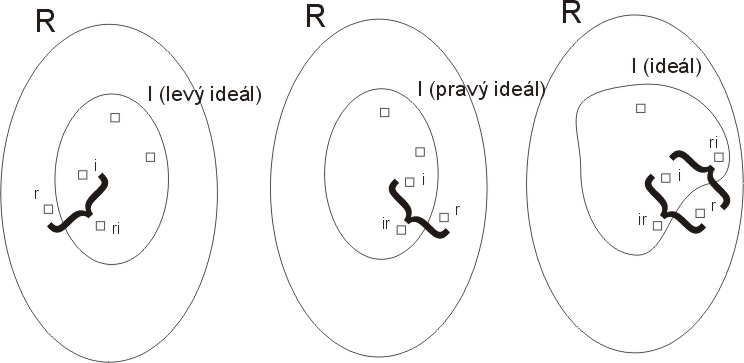
\includegraphics[scale=0.4]{matematika/obrazky/ideal}
\end{center}
\end{e}

\begin{e}{P��klady}{0}{0}
P��klady ide�l�:
\begin{pitemize}
    \item $\{0\}$ a $R$ jsou (nevlastn�, trivi�ln�) ide�ly v ka�d�m okruhu $R$
    \item Sud� cel� ��sla tvo�� ide�l v okruhu $\Whole$, podobn� to plat� pro $n\Whole$, kde $n$ je p�irozen�.
    \item Mno�ina polynom� d�liteln�ch $x^2+1$ je ide�lem v okruhu v�ech polynom� s 1 prom�nnou a re�ln�mi koeficienty
    \item Mno�ina matic $n\times n$ s nulov�m posledn�m sloupcem vpravo je lev� ide�l v okruhu v�ech matic $n\times n$, nen� to ale prav� ide�l (podobn� s ��dky a opa�n�mi ide�ly)
\end{pitemize}
\end{e}


\begin{e}{Pozn�mka}{0}{Vlastnosti ide�l�}
Pr�nik (lev�ch, prav�ch) ide�l� tvo�� op�t (lev�, prav�) ide�l. \emph{Ide�l generovan� podmno�inou} $A$ okruhu $R$ je pr�nik v�ech ide�l� v $R$, kter� $A$ obsahuj�. V�echny ide�ly nad n�jak�m okruhem s pr�niky a ide�ly generovan�mi sjednocen�m tvo�� �pln� svaz.

$I$ je \emph{maxim�ln� ide�l}, pokud je netrivi�ln� a ��dn� jin� netrivi�ln� ide�l nen� jeho nevlastn� nadmno�inou. \emph{Prvoide�l} $P$ v okruhu $R$ je takov� ide�l, �e pro ka�d� $a,b\in R$, pokud je $ab\in P$, potom mus� b�t $a\in P$ nebo $b\in P$. Prvoide�ly maj� v n�kter�ch ohledech podobn� vlastnosti jako prvo��sla. Ka�d� max.ide�l je prvoide�l.(fakt??)
\\\\
Je-li ide�l vlastn�, pak neobsahuje $1$. Ka�d� ide�l je nepr�zdn�, proto�e jako podgrupa $(R,+,-,0)$ mus� obsahovat $0$. 
\\\\
Ide�l n$\mathbb{Z}$ je prvoide�l $\Leftrightarrow$ n je prvo��slo.
\begin{center}
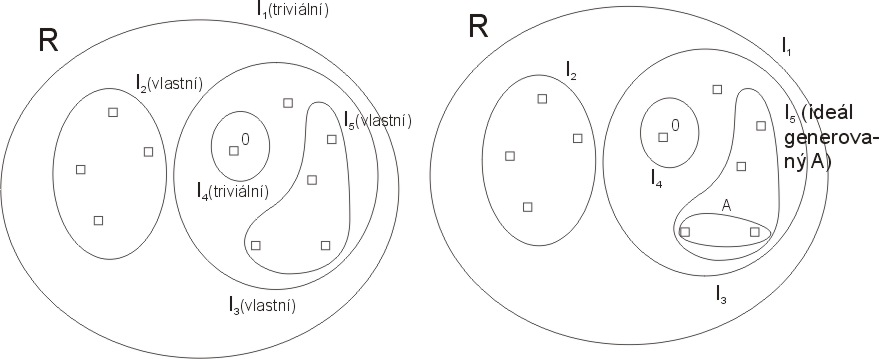
\includegraphics[scale=0.5]{matematika/obrazky/vlastni_ideal}
\end{center}
\end{e}

\begin{reportN}{Kral} zda lze z definice neutr�ln�ho prvku, kter� je nadefinovan� e*x=x vyvodit i x*e=x, kdy� je * jen asociativn� (podle me nelze, te definici
se rika levy neutralni prvek)
\end{reportN}
\begin{reportN}{IP 21.6.2011} Vypsat v�echny podgrupy grupy $S_3$ (grupa permutac� na 3 prvc�ch) a jejich index.
Definovat index podgrupy a vyslovit vitu o vztahu velikosti grupy, jej� podgrupy a indexu (to m�la b�t Lagrangeova vita). 
\end{reportN}
\begin{reportN}{�emli�ka KSI} Grupa, okruh, teleso. Definice, priklady
nakreslil jsem na papir toto:(obrazek dedicnosti) 
a podebatovali jsme 
\end{reportN}
\begin{reportN}{Fiala} Normalni grupy a faktorgrupy -  normalni grupu jsem dal dohromady, jednoduchy priklad taky. U faktorgrupy jsem poradne nevedel, co to je [docela ostudne po vsech tech vetach o homomorfismu/isomorfismu apod z Algebry I], malem jsem byl proto odejit, kvuli ostatnim znamkam ale 3- 
\end{reportN}
\begin{reportN}{Matousek} grupy, hodne prikladu + normalni podgrupy a priklady (normalnich a nenormalnich) definici grupy jsem tak nejak popsal pres algebru a monoid (u monoidu jsem zapomel na asociativitu, na to se me pak zeptal), priklady grup jsem nejake vedel, normalnich podgrup ani moc ne, ale trosku mi pomohl a nejak jsme to dali dohromady  
\end{reportN}

\subsection{Homomorfismy grup}

\subsubsection*{Obecn� tvrzen� o homomorfismech algeber (plat� i pro grupy)}

\begin{e}{Definice}{0}{homomorfismus}
O zobrazen� $f: A\to B$ �ekneme, �e je \emph{slu�iteln�} s operac� $\alpha$, pokud pro ka�d� $a_1,\dots a_n\in A$ plat� $f(\alpha_{(A)}(a_1, ... a_n )) = \alpha_{(B)}( f(a_1), ... f(a_n) )$. Pro algebry stejn�ho typu (se stejn�m po�tem operac� stejn� arity) je zobrazen� $f:A\to B$ \emph{homomorfismus}, pokud je slu�iteln� se v�emi jejich operacemi.

Bijektivn� homomorfismus se naz�v� \emph{isomorfismus}, algebry stejn�ho typu jsou \emph{isomorfn�}, existuje-li mezi nimi aspo� 1 isomorfismus.
\begin{center}
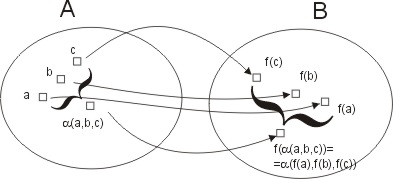
\includegraphics[scale=0.5]{matematika/obrazky/slucitelnost_s_operaci}
\\Slu�itelnost s operac� - pokud to nejprve zobraz�m a pak aplikuji operaci, mus� mi vyj�t to sam� jako kdybych nejprve pou�il operaci a zobrazil a� v�sledek. \end{center}
\end{e}

\begin{e}{Pozn�mka}{0}{Vlastnosti homomorfism�}
Slo�en� homomorfism� je homomorfismus. Je-li $f$ bijekce a homomorfismus, je $f^{-1}$ taky homomorfismus.
\end{e}

\begin{e}{Definice}{0}{p�irozen� projekce, j�dro zobrazen�}
\emph{P�irozen� projekce} mno�iny $A$ podle kongruence $\rho$ je $\pi_{\rho}: A\rightarrow A/\rho$, kde    $\pi_{\rho}(a) = [a]_{\rho}$. Pro zobrazen� $f:A\to B$ se \emph{j�dro zobrazen�} definuje jako relace $\ker f$ p�edpisem $(a_1,a_2)\in \ker f \equiv^{def} f(a_1) = f(a_2)$.

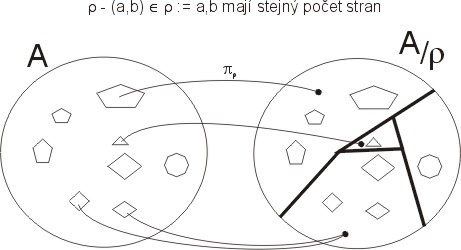
\includegraphics[scale=0.65]{matematika/obrazky/prirozena_projekce}
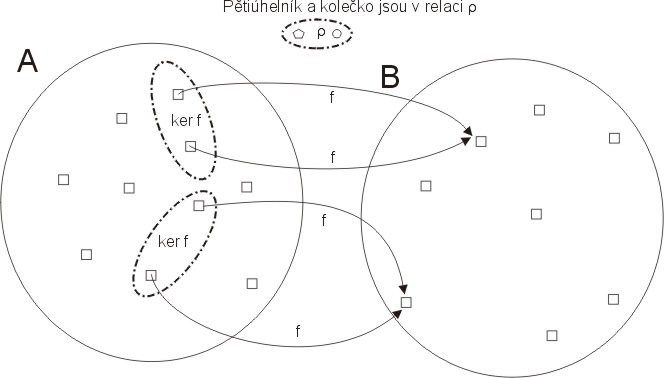
\includegraphics[scale=0.45]{matematika/obrazky/kerf}
\\P�irozen� projekce prost� zobraz� prvek na jeho t��du ekvivalence.
\end{e}

\begin{e}{Pozn�mka}{0}{homomorfismy a kongruence}
Pro ka�dou kongruenci $\rho$ na libovoln� algeb�e $A$ je p�irozen� projekce $\pi_{\rho}:A\to A/\rho$ homomorfismus.
\end{e}

\begin{e}{V�ta}{0}{O homomorfismu}
Nech� $f:A\to B$ je homomorfismus algeber stejn�ho typu a $\rho$ kongruence na $A$. Potom:
\begin{penumerate}
    \item existuje homomorfismus $g:A/\rho\to B$ takov�, �e $f=g\pi_{\rho}$  pr�v� kdy� $\rho\subseteq \ker f$,\footnote{p�irozen� projekce je taky homomorfismus}
    \item $g$ je nav�c isomorfismus, pr�v� kdy� $f$ je na (surjekce) a $\rho = \ker f$.\footnote{surjekce je rozbrazen� na celou c�lovou mno�inu}
\end{penumerate}
\end{e}

\begin{e}{Definice}{0}{faktor-ekvivalence} $\rho\subseteq\sigma$ 2 ekvivalence na $A$. Pak \emph{$\sigma$/$\rho$ - faktor-ekvivalence}
je relace definovan�: $([a]_{\rho},[b]_{\rho})\in\sigma/\rho\ \stackrel{\mathrm{def}}\equiv (a,b)\in\sigma$.
\\\\
Relace \emph{$\rho$ slu�iteln� s $\alpha$}, pak $\alpha$ na A/$\rho$
def.: $\alpha([a_1]_{\rho},... [a_n]_{\rho}) = [ \alpha(a_1, ... a_n) ]_{\rho}$.
Kongruence $\rho$ na A, pak stejn�m zp�sobem def. na A/$\rho$ strukturu algebry.
\begin{center}
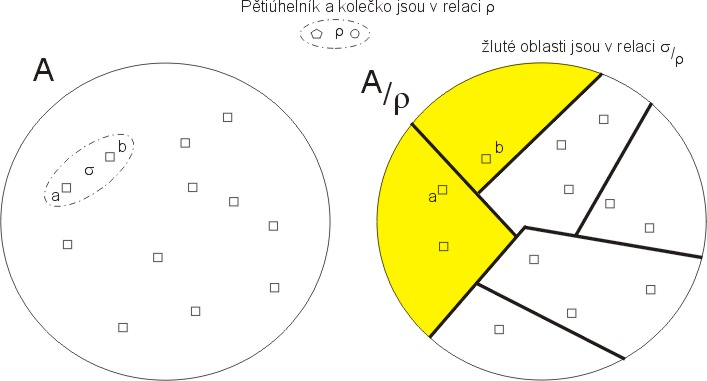
\includegraphics[scale=0.5]{matematika/obrazky/relace_sigma_ro}
\\�esky �e�eno, sna��m se d�t do relace chl�vky, tak�e se neprve mrknu jestli jsou v relaci jejich reprezentanti.  
\end{center}
\end{e}

\begin{e}{V�ta}{0}{V�ty o isomorfismu}
\begin{penumerate}
    \item Nech� $f:A\to B$ je homomorfismus algeber stejn�ho typu, pak $f(A)$ je podalgebra $B$ a $^{A}/_{\ker f}$ je isomorfn� algeb�e $f(A)$.
    \item Nech� $\rho\subseteq\eta$ jsou dv� kongruence na algeb�e $A$. Pak algebra $^{(A/\rho)}/_{(\eta/\rho)}$ je isomorfn� algeb�e $^A/_{\eta}$.
\end{penumerate}
\end{e}

\subsubsection*{Homomorfismy grup}

\begin{e}{V�ta}{0}{O homomorfismu grup}
Je-li zobrazen� $f:G\to H$, kde $G,H$ jsou grupy, slu�iteln� s bin. operac�, pak je homomorfismus. (D�kaz: nejd��v dok�zat slu�itelnost s \uv{$e$} a pak \uv{$^{-1}$}, oboje p��mo z definice grupy.)
\end{e}

\begin{e}{Definice}{0}{mocnina prvku}
V grup� lze definovat \emph{$g^n$} (kde $n\in\Whole$) jako: 
\begin{pitemize}
    \item $g^0=1$, 
    \item $g^{n+1}=g\cdot g^n\ \ (n>0)$, 
    \item $g^{n}=(g^{-1})^{-n}\ \ (n<0)$.
\end{pitemize}

\emph{Mocninn� podgrupa} grupy $G$ je potom cyklick� podgrupa -- pro n�jak� prvek $g\in G$ jde o mno�inu $\{\dots,g^{-1},g^0,g,g^2,\dots\}$.
\end{e}

\begin{e}{Pozn�mka}{0}{O mocnin� prvku}
Je-li zobrazen� $\varphi:\Whole\to G$ definov�no p�edpisem  $\varphi_g (n) = g^{n}$ (tj. jde o mocniny prvku $g$), kde $g\in (G,\cdot,^{-1},1)$, pak je $\varphi$ grupov� homomorfismus $(\Whole,+,-,0)$ a $(G,\cdot,^{-1},1)$.
\end{e}

\begin{e}{Pozn�mka}{0}{Vlastnosti cyklick�ch grup}
Nech� grupa $(G,\cdot,^{-1},1)$ je cyklick�. Potom plat�:
\begin{penumerate}
    \item Je-li $G$ nekone�n�, pak $G\simeq(\Whole,+,-,0)$ (je isomorfn� s cel�mi ��sly).
    \item Je-li $n = |G|$ kone�n�, pak $(G,\cdot,^{-1},1)\simeq(\Whole_n,+,-,0)$ (je isomorfn� s grupou zbytkov�ch t��d odpov�daj�c� velikosti).
\end{penumerate}
\end{e}

\newpage
\subsection{D�litelnost a ireducibiln� rozklady polynom�}

\begin{center}
Zdroje n�sleduj�c�ch sekc�: texty J. �emli�ky k p�edn�ce Algebra II\\
\texttt{http://www.karlin.mff.cuni.cz/\~{}zemlicka/cvic6-7/algi.htm}\\
a skripta R. El Bashira k p�edn�ce Algebra I a II pro matematiky\\
\texttt{http://www.karlin.mff.cuni.cz/\~{}bashir/}\\
\end{center}

\subsubsection*{Nejv�t�� spole�n� d�litel}

\begin{e}{Definice}{0}{Komutativn� monoid s kr�cen�m}
Monoid $(S,\cdot, 1)$ je \emph{komutativn� monoid s kr�cen�m}, pokud operace \uv{$\cdot$} je komutativn� a nav�c spl�uje $$\forall a,b,c\in S: a\cdot c=b\cdot c\implies a = b$$
\end{e}

\begin{e}{Definice}{0}{D�len�, asociovanost}
O prvc�ch $a,b$ n�jak�ho komutativn�ho monoidu s kr�cen�m $S$ �ekneme, �e \emph{$a$ d�l� $b$} ($a|b$, $b$ je d�liteln� $a$), pokud existuje takov� $c\in S$, �e $b=a\cdot c$. �ekneme, �e \emph{$a$ je asociov�n s $b$} ($a||b$), jestli�e $a|b$ a z�rove� $b|a$.
\end{e}

\begin{e}{Definice}{0}{Obor integrity}
\emph{Obor integrity} je takov� komutativn� okruh $(R,+,\cdot,-,0,1)$, ve kter�m plat�, �e $a\cdot b=0$ implikuje $a=0$ nebo $b=0$.
\end{e}

\begin{e}{P��klady}{0}{0}
\begin{penumerate}
    \item $(\Whole,+,\cdot,-,0,1)$ je obor integrity.
    \item Pro ka�d� obor integrity $(R,+,\cdot,-,0,1)$ je $(R\setminus\{0\},\cdot,1)$ komutativn� monoid s kr�cen�m (\uv{multiplikativn� monoid}).
\end{penumerate}
\end{e}

\begin{e}{Pozn�mka}{0}{Vlastnosti \uv{$||$}}
V komutativn�m monoidu s kr�cen�m $(S,\cdot,1)$ plat� pro $a,b\in S$, �e $a||b$, pr�v� kdy� existuje invertibiln� prvek $u$ z $S$  takov�, �e $a=b\cdot u$. Relace \uv{$||$} tvo�� kongruenci na $S$ a faktoralgebra $(S/||,\cdot,[1]_{||})$ podle t�to kongruence je tak� komutativn� monoid s kr�cen�m (relace \uv{$|$} na n�m tvo�� uspo��d�n�).
\end{e}


\begin{e}{Definice}{0}{Nejv�t�� spole�n� d�litel}
M�jme komutativn� monoid s kr�cen�m $(S,\cdot,1)$ a v n�m prvky $a_1,\dots,a_n$. Prvek $c$ nazveme nejv�t��m spole�n�m d�litelem prvk� $a_1,\dots,a_n$, pokud $c|a_i$ pro v�echna $i\in\{1,\dots,n\}$ a z�rove� libovoln� prvek $d\in S$, kter� d�l� v�echna $a_i$ d�l� i $c$. P�eme $\NSD(a_1,\dots,a_n)=c$. 

Stejn� se definuje nejv�t�� spole�n� d�litel pro obory integrity (bereme obor integrity $(R,+,\cdot,-,1,0)$ jako komutativn� monoid s kr�cen�m $(R\setminus\{0\},\cdot,1)$).
\end{e}

\begin{e}{Definice}{0}{Ireducibiln� prvek, prvo�initel�}
Prvek $c$ komutativn�ho monoidu s kr�cen�m $(S,\cdot,1)$ nazveme \emph{ireducibiln�m}, pokud $c$ nen� invertibiln� a z�rove� $c=a\cdot b$ pro n�jak� $a,b\in S$ v�dy implikuje $c||a$ nebo $c||b$. Prvek $c$ nazveme \emph{prvo�initelem}, pokud nen� invertibiln� a z�rove� $c|a\cdot b$ pro $a,b\in S$ v�dy implikuje $c|a$ nebo $c|b$. 

Na oborech integrity se prvo�initel� a ireducibiln� prvky definuj� stejn�.
\end{e}


\begin{e}{V�ta}{0}{Vlastnosti $\NSD$}
V komutativn�m monoidu s kr�cen�m $(S,\cdot,1)$ pro prvky $a,b,c,d,e$ plat�:
\begin{penumerate}
    \item $d=\NSD(a,b)\ \&\ e=\NSD(a\cdot c,b\cdot c) \implies (d\cdot c)||e$.
    \item $1=\NSD(a,b)\ \&\ a|(b\cdot c)\ \&$ $\NSD(a\cdot c,b\cdot c)$ existuje $\implies$ $a|c$.
\end{penumerate}
\end{e}

\begin{e}{V�ta}{0}{Vlastnosti prvo�initel�}
V komutativn�m monoidu s kr�cen�m je ka�d� prvo�initel ireducibiln�. Pokud nav�c pro ka�d� dva jeho prvky existuje nejv�t�� spole�n� d�litel, je ka�d� ireducibiln� prvek prvo�initelem.
\end{e}

\subsubsection*{Polynomy}

\begin{e}{Definice}{0}{Okruh polynom�}
Nad okruhem $(R,+,\cdot,-,0,1)$ a monoidem $(M,\cdot,e)$ definujme okruh $(R[M],+,\cdot,-,0,1)\text{,}$ kde:
\begin{pitemize}
    \item $R[M]=\{ p:M\to R | \{m|p(m)\neq 0\} \text{ je kone�n� } \}$
    \item prvek $p\in R[M]$ se d� zapsat jako $p=\sum_{m\in M}(p(m).m)$
    \item operace \uv{$+$} je definov�na jako: $p+q=\sum_{m\in M}((p(m)+q(m)).m)$
    \item \uv{$\cdot$} je definov�no n�sledovn�: $p\cdot q=\sum_{m\in M}((\sum_{r\cdot s=m} p(r)\cdot q(s)).m)$
    \item dal�� operace:
    \begin{pitemize}
        \item $-p=\sum_{m\in M}(-p(m))\cdot m$,
        \item $0=\sum_{m\in M}0.m$,
        \item $1=(1\cdot e)+\sum_{m\in M\setminus\{e\}}0.m$.
    \end{pitemize}
\end{pitemize}
\par
Pro okruh $(R,+,\cdot,-,0,1)$ a monoid $(\Nat_0,+,0)$ nez�porn�ch cel�ch ��sel se s��t�n�m nazveme $R[\Nat_0]$ (ozna�me $R[x]$) \emph{okruh polynom� jedn� nezn�m�}. Jeho prvky potom nazveme \emph{polynomy} a budeme je zapisovat ve tvaru $p=\sum_{n\in\Nat_0}p(n).x^n$. 
% ta tecka tady fakt ma smysl, sice je mnohem osklivejsi ale jde o jinou operaci nez nasobeni v tom
% okruhu !
\end{e}

\begin{e}{Pozn�mka}{0}{0}
$R[x]$ nad okruhem $R$ je obor integrity, pr�v� kdy� $R$ je obor integrity.
\end{e}


\begin{e}{Definice}{0}{Stupe� polynomu}
Pro polynom $p$ v okruhu $R[x]$ nad $(R,+,\cdot,-,0,1)$ definujeme \emph{stupe� polynomu} ($\deg p$, $\st p$) n�sledovn�: $$\deg p=\begin{cases}
\text{nejv�t�� }n\in\Nat_0:p(n)\neq 0\text{, je-li }p\neq 0\\
-1\text{, je-li }p=0
\end{cases}$$
\end{e}

\begin{e}{Pozn�mka}{0}{Vlastnosti $\deg p$}
V okruhu $R[x]$ nad $(R,+,\cdot,-,0,1)$ plat� pro $p,r\in R[x]$:
\begin{pitemize}
    \item $\deg -p = \deg p$
    \item $\deg (p+q) = \max(\deg p,\deg q)$
    \item Je-li $p\neq 0, q\neq 0$, pak $\deg (p\cdot q)\leq \deg p + \deg q$ (na oborech integrity plat� rovnost)
\end{pitemize}
\end{e}

\begin{e}{V�ta}{0}{D�len� polynom� se zbytkem}
Nech� jsou na oboru integrity $(R[x],+,\cdot,-,0,1)$ (nad oborem integrity $R$) d�ny prvky $a,b\in R[x]$. Nech� nav�c $m=\deg b\geq 0$ a $b_m$ je invertibiln� v $R$. Potom existuj� jednozna�n� ur�en� polynomy $q,r\in R[x]$ takov�, �e $a=b\cdot q+r$ a $\deg r<\deg b$.
\end{e}

\begin{e}{Pozn�mka}{0}{0}
Polynom $q$ je \emph{pod�l} polynom� $a$ a $b$, polynom $r$ je \emph{zbytek} p�i d�len�.
\end{e}

\subsubsection*{Nejv�t�� spole�n� d�litel}

\begin{e}{Definice}{0}{Eukleidovsk� obor integrity}
Obor integrity $(R,+,\cdot,-,0,1)$ je \emph{eukleidovsk�}, jestli�e existuje zobrazen� $\nu:R\to \Nat_0\cup\{-1\}$ (\emph{eukleidovsk� funkce}), kter� pro ka�d� $a,b\in R$ spl�uje:
\begin{penumerate}
    \item Jestli�e $a|b$ a $b\neq 0$, pak $\nu(a)\leq\nu(b)$
    \item Pokud $b\neq 0$, existuj� $q,r\in R$ takov�, �e $a=b\cdot q + r$ a $\nu(r)<\nu(b)$
\end{penumerate}
\end{e}

\begin{e}{Pozn�mka}{0}{0}
Je-li $(T,+,\cdot,-,0,1)$ n�jak� komutativn� t�leso, pak $T[x]$ je eukleidovsk�m oborem integrity s eukleidovskou funkc� danou stupn�m polynom�. P��kladem eukleidovsk�ho oboru integrity jsou nap�. i cel� ��sla (se s��t�n�m, n�soben�m, un�rn�m minus, jedni�kou a nulou), kde eukleidovsk� funkce je funkce absolutn� hodnoty prvku.
\end{e}

\begin{e}{Algoritmus}{0}{Eukleid�v algoritmus}
Na eukleidovsk�m okruhu $R$ s eukleidovskou funkc� $\nu$ pro dva prvky $a_0,a_1\in R\setminus\{0\}$ najdeme nejv�t�� spole�n� d�litel n�sleduj�c�m postupem:
\begin{pitemize}
    \item Je-li $i\geq 1$ a $a_i\not |\ a_{i-1}$, vezmeme $a_{i+1}\in R$ takov�, �e $a_{i-1}=a_i\cdot q_i+a_{i+1}$ pro n�jak� $q_i$ a $\nu(a_{i+1})<\nu(a_i)$. $i$ zv���me o $1$ a pokra�ujeme dal�� iterac� \footnote{znak $\not |\ $ znamen� ned�l� }.
    \item Je-li $i\geq 1$ a $a_i|a_{i-1}$, potom $a_i = \NSD(a_0,a_1)$ a v�po�et kon��.
\end{pitemize}
D� se dok�zat, �e se v�po�et zastav� a kroky jsou dob�e definovan� (lze nal�zt $a_{i+1}$ a $q_i$), tedy libovoln� dva polynomy maj� nejv�t��ho spole�n�ho d�litele.
\end{e}

\begin{e}{Pozn�mka}{0}{0}
Nejv�t�� spole�n� d�litel je v polynomech $R[x]$ ur�en a� na asociovanost ($||$) jednozna�n�. Pro asociovan� polynomy $p,q$ v�dy plat�, �e $\deg p=\deg q$ a $p=r\cdot q$ pro n�jak� $r\in R$.
\end{e}

\begin{reportN}{Kratochv�l} Dal mi jeste prakticky priklad na delitelnost, jestli jeden zadany polynom je delitelem druheho (ze by zachrana? bo toto pocitaji decka nekde v sexte na gymplu :D). Tak priklad spocitan, k tomu stranka teorie. Myslim, ze jsem nektere hlavni veci mel, NSD, Eukleida, co je to koren a rozklad, co je ireducibilni polynom a take to, ze v C - narozdil od R - ma kazdy polynom koren a polynom stupne $\geq2$ je vzdy reducibilni. No a pak zacal. :) Chtel mimo jine "nejak popsat" vsechny ireducibilni polynomy v R,Q a C. No tady jsem to moc nedaval, dost mi pomahal... Spolecnymi silami jsme to nakonec dali dohromady (pro zvedavce spr. odpoved: polynom je ireducibilni v C $\Leftrightarrow$ je stupne 1, ireducibilni v R $\Leftrightarrow$ je stupne 1 nebo 2, a v Q pro libovolne n existuje ireducibilni - napr $x^n-2$) 
\end{reportN}

\subsection{Rozklady polynom� na ko�enov� �initele}

\subsubsection*{Rozklady polynom�}

\begin{e}{Pozn�mka}{0}{Ireducibiln� polynomy}
Polynom je ireducibiln�, pokud nen� sou�inem dvou polynom� ni���ch stup�� a jeho stupe� je v�t�� nebo roven jedn�. V�echny polynomy stupn� 1 jsou ireducibiln�. Jedin�mi d�liteli ireducibiln�ho polynomu jsou asociovan� polynomy a nenulov� skal�ry (tj. polynomy stupn� 0).
\end{e}


\begin{e}{V�ta}{0}{Rozklad polynomu}
Ka�d� polynom stupn� alespo� 1 m� a� na asociovanost jednozna�n� rozklad na sou�in ireducibiln�ch polynom�. \\\textit{D�kaz existence:} indukc� podle $\deg p$ -- najdeme v�dy d�litel $p$ nejmen��ho mo�n�ho kladn�ho stupn�, vyd�l�me a pokra�ujeme, dokud nedostaneme polynom, kter� nem� d�litel kladn�ho stupn� men��ho ne� je jeho vlastn�.
\end{e}


\begin{e}{Definice}{0}{Dosazov�n� do polynom�}
Nech� $(S,+,\cdot,-,0,1)$ je okruh, $R$ jeho podokruh ($R\subset S$) a nech� $\alpha\in S$. Potom zobrazen� $j_\alpha : R[x]\to S$, dan� p�edpisem $j_\alpha(\sum_{n\in\Nat_0}a_n.x^n) = \sum_{n\in\Nat_0}a_n\cdot\alpha^n$ je okruhov� homomorfismus. Naz�v� se \emph{dosazovac� homomorfismus}.
\end{e}

\begin{e}{Pozn�mka}{0}{Dosazovan� a $\deg p$}
Pro obor integrity $R[x]$ nad oborem integrity $(R,+,\cdot,-,0,1)$ je polynom $p[x]$ invertibiln�, pr�v� kdy� $\deg p=0$ a $j_0(p)=p(0)$ je invertibiln� na $R$.
\\Nap�.: kdy� m�m polynom $(x^n+...)$, kde $n>0$, ni��m ho u� nem��u vyn�sobit,
abych z�skal 1.
\end{e}

\begin{e}{Definice}{0}{Ko�en polynomu}
Pro okruh $(S,+,\cdot,-,0,1)$ a jeho podokruh $R$ je \emph{ko�en polynomu} $p\in R[x]$ takov� $\alpha\in S$, �e $j_\alpha(p)=p(\alpha)=0$ (p�i dosazen� $\alpha$ se polynom $p$ zobraz� na $0$).
\end{e}

\begin{e}{Definice}{0}{Ko�enov� �initel, rozklad}
Je-li $a=c\cdot p_1^{k_1}\cdot\dots p_n^{k_n}$ rozklad polynomu $p\in R[x]$ na ireducibiln� polynomy, potom \emph{ko�enov�m �initelem} polynomu $p$ nazveme takov� $p_i$, kter� je ve tvaru $x-\alpha$ (tedy stupn� 1 s koeficienty $1$ a $\alpha$). �ekneme, �e polynom $p\in R[x]$ se \emph{rozkl�d� na ko�enov� �initele} v $R[x]$, jestli�e existuje takov� jeho rozklad na ireducibiln� polynomy, �e v�echny $p_i$ jsou ko�enov� �initele. Potom nazveme $k_i$ \emph{n�sobnostmi ko�en�}.
\end{e}

\begin{e}{V�ta}{0}{ko�en a ko�enov� �initel}
Na oboru integrity $R[x]$ nad oborem integrity $R$ je $\alpha\in R$ ko�enem polynomu $p\in R[x],p\neq 0$, pr�v� kdy� $(x-\alpha)|p$. 
\end{e}

\subsubsection*{Komplexn�, re�ln� a racion�ln� polynomy}

\begin{e}{Definice}{0}{Algebraicky uzav�en� t�leso}
Nech� $T$ je t�leso a $S$ jeho nadt�leso. Prvek $a\in S$ je \emph{algebraick�} nad $T$, pokud existuje n�jak� nenulov� polynom z $T[x]$, jeho� je $a$ ko�enem. Pokud ��dn� takov� polynom neexistuje, naz�v� se prvek \emph{transcendentn�}. T�leso $T$ je \emph{algebraicky uzav�en�}, pokud v�echny nad n�m algebraick� prvky jsou i jeho prvky (jsou v n�m obsa�eny).
\end{e}

\begin{e}{Pozn�mka}{0}{0}
Ka�d� polynom v okruhu polynom� o jedn� nezn�m� nad algebraicky uzav�en�m t�lesem se rozkl�d� na ko�enov� �initele.
\end{e}

\begin{e}{V�ta}{0}{Z�kladn� v�ta algebry}
T�leso $\Complex$ komplexn�ch ��sel je algebraicky uzav�en� \footnote{$\Real$
nebo $\mathbb{Q}$ ne}.
\end{e}

\begin{e}{D�sledek}{0}{0}
Proto m� ka�d� polynom $p(x)\in\Complex[x]$ stupn� alespo� 1 v $\Complex[x]$ rozklad tvaru $p(x)=a(x-\beta_1)^{k_1}\cdot\dots\cdot(x-\beta_s)^{k_s}$, kde $\sum_{i=1}^s k_i=n$ a $\beta_i$ jsou navz�jem r�zn�.
\end{e}

\begin{e}{V�ta}{0}{Komplexn� sdru�en� ko�eny v $\Complex$}
M�-li polynom $p$ nad $\Complex[x]$ s re�ln�mi koeficienty ($a_i\in\Real$) ko�en $\alpha\in\Complex$, pak je jeho ko�enem i $\overline{\alpha}$, tedy ��slo komplexn� sdru�en� s $\alpha$.
\end{e}

\begin{e}{D�sledek}{0}{0}
Polynom $p(x)\in\Real[x]$ stupn� alespo� 1 m� v $\Real[x]$ rozklad tvaru 
$$p(x)=a(x-\alpha_1)^{k_1}\cdot\dots(x-\alpha_r)^{k_r}\cdot(x^2-a_1 x+b_1)^{l_1}\cdot\dots(x^2-a_s x+b_s)^{l_s}$$
a polynomy $x^2+a_j x+b_j$, kde $j\in\{1,\dots s\}$ maj� za ko�eny dvojice komplexn� sdru�en�ch ��sel (kter� nejsou �ist� re�ln�). Nav�c $\deg p=k_1+\dots+k_r+2(l_1+\dots+l_s)$.
\\V $\Real$ existuj� ireducibiln� polynomy stupn� max 2!
\end{e}

\begin{e}{D�sledek}{0}{0}
Ka�d� polynom v $\Real[x]$ lich�ho stupn� m� alespo� jeden re�ln� ko�en.
\end{e}

\begin{e}{V�ta}{0}{Ireducibiln� polynomy v $\Rational$}
V $\Rational[x]$ existuj� ireducibiln� polynomy libovoln�ho stupn� v�t��ho nebo rovn�ho jedn� (tj. ne v�dy existuje rozklad na ko�enov� �initele, ani rozklad na polynomy stupn� max. 2 jako v re�ln�ch ��slech).
\end{e}

\subsection{N�sobnost ko�en� a jejich souvislost s derivacemi mnoho�lenu}

\begin{e}{V�ta}{0}{o po�tu ko�en�}
Ka�d� nenulov� polynom $p\in R[x]$, kde $R[x]$ je okruh polynom� nad oborem integrity $(R,+,\cdot,-,0,1)$, m� nejv��e $\deg p$ ko�en� (plyne z vlastnost� $\deg p$).
\end{e}

\begin{e}{Definice}{0}{v�cen�sobn� ko�en}
Pro komutativn� okruh $(R,+,\cdot,-,0,1)$ a polynom $p\in R[x]$ je $\alpha\in R$ \emph{v�cen�sobn� ko�en}, pokud polynom $(x-\alpha)(x-\alpha)$ d�l� $p$.
\end{e}

\begin{e}{Definice}{0}{Derivace polynomu}
Pro polynom $p=\sum_{i\geq 0}a_i x^i$ z okruhu polynom� $R[x]$ nad komutativn�m okruhem $(R,+,\cdot,-,0,1)$ definujeme \emph{derivaci} ($p'$, $p'\in R[x]$) p�edpisem $$p'=\sum_{i\geq 0}(i+1)a_{i+1}x^i$$
\end{e}

\begin{e}{Pozn�mka}{0}{Vlastnosti derivace}
Pro okruh $(R,+,\cdot,-,0,1)$, prvek $\alpha\in R$ a polynomy $p,q\in R[x]$ plat�:
\begin{pitemize}
    \item $(p+q)'=p'+q'$
    \item $(\alpha p)'=\alpha p'$
    \item $(p\cdot q)' = p'\cdot q + p\cdot q'$
\end{pitemize}
\end{e}

\begin{e}{V�ta}{0}{derivace a v�cen�sobn� ko�en}
Nad oborem integrity $(R,+,\cdot,-,0,1)$ bu� $p\in R[x]$ polynom. Je-li $\alpha\in R$ jeho ko�en, pak $\alpha$ je v�cen�sobn� ko�en, pr�v� kdy� je $\alpha$ ko�enem $p'$.
\end{e}

\begin{e}{Definice}{0}{Charakteristika oboru integrity}
Pro obor integrity $(R,+,\cdot,-,0,1)$ definujeme \emph{charakteristiku oboru integrity $char R$} jako
\begin{pitemize}
    \item $0$ (nebo n�kdy $\infty$), pokud cyklick� podgrupa grupy $(R,+,0)$ generovan� prvkem $1$ je nekone�n�.
    \item $p$, pokud cyklick� pogrupa grupy $(R,+,0)$ generovan� jedni�kou m� kone�n� ��d $p$.
\end{pitemize}
\end{e}

\begin{e}{P��klad}{0}{0}
$char \Complex= char \Real=char \mathbb{Q}=char \mathbb{Z}=0$
\\$char \Whole_p=p$
\end{e}

\begin{e}{V�ta}{0}{derivace sni�uje stupe� polynomu}
Nad oborem integrity charakteristiky $0$ $(R,+,\cdot,-,0,1)$ bu� $p$ polynom ($p\in R[x]$) stupn� $n>0$. Potom $p'$ je polynom stupn� $n-1$.
\end{e}

\begin{e}{V�ta}{0}{derivace a n�sobn� ko�en}
Nad t�lesem charakteristiky $0$ $(T,+,\cdot,-,0,1)$ bu� $p$ polynom ($p\in T[x]$) stupn� alespo� 1. Potom prvek $\alpha\in U$, kde $U$ je n�jak� nadt�leso $T$, je $k$-n�sobn�m ko�enem $p$, pr�v� kdy� plat� ob� n�sleduj�c� podm�nky:
\begin{pitemize}
    \item $p(\alpha)=j_{\alpha}(p)=0$, $p'(\alpha)=0$, $\dots$ $p^{(k-1)}(\alpha)=0$
    \item $p^{(k)}(\alpha)\neq 0$
\end{pitemize}
\end{e}

\begin{e}{V�ta}{0}{derivace a nejv�t�� spole�n� d�litel}
M�jme t�leso $(T,+,\cdot,-,0,1)$ charakteristiky $0$ a nad n�m polynom $p\in T[x]$ stupn� alespo� $1$. Potom plat�:
\begin{pitemize}
    \item Pokud $\NSD(p,p')=1$, pak $p$ nem� ��dn� v�cen�sobn� ko�en.
    \item Ka�d� $k$-n�sobn� ko�en $p$ je $(k-n)$-n�sobn�m ko�enem $n$-t� derivace $p$.
    \item Polynom $q\in R[T]$ takov�, �e $q\cdot\NSD(p,p')=p$ m� stejn� ko�eny jako $p$, ale jednoduch�.
\end{pitemize}
\end{e}

\begin{e}{V�ta}{0}{0}
Nech� $(R,+,\cdot,-,0,1)$ je obor integrity a jeho charakteristika ned�l� ��slo $n\in \mathbb{N}$. Potom polynomy $x^n-1$ a $x^{n+1}-x$ v $R[x]$ nemaj� v�cen�sobn� ko�en.
\end{e}

\begin{reportN}{�emlieka} souvislost derivace s viacnasobnym korenom polynomu (tam odo mna chcel zemlicka aj priklad pouzitia a naviedol ma na dake specialne sposoby vypoctu korenov polynomov) 
\end{reportN}
\begin{reportN}{Zahradnik} mi dal suvislost nasobnosti korena a derivacie polynomu. K tej druhej otazke som napisal akurat 2 vety a to im na zaciatok stacilo...
\end{reportN}
\begin{reportN}{Majerech} Druh� ot�zka algebra... no todle se mi moc nel�bilo ... ale ot�zky byly je�te z�ludnej��....
Mejme re�ln� polynom, o kter�m v�te, �e ��dn� dva koreny nemaj� stejnou n�sobnost
\\a) Kolik m� takov� polynom re�ln�ch korenu? m� v�echny koreny re�ln� nebo? libovoln� komplexn� koren a jeho sdru�en� part�k maj� shodnou n�sobnost 
toto je trivialita... ale prij�t na to... mi trvalo... pul hodiny... je to divoce formulovan�...
\\b)Najdete v�echny koreny tohoto polynomu /presne/
\\Prvn� pozorov�n�: kdy� je kooen n�sobn� tak je kooenem derivace...
\\Druh� pozorov�n�: derivace puvodn�ho polynomu je tvaru
\\$Q'(x)=P(x)*balast0$
\\puvodn� polynom je tvaru
\\$Q(x)=P(x)*balast1$
\\Tret� pozorov�n�: P(x) je NSD Q(x) a Q'(x), kde P(x) je produkt tech n�sobn�ch korenu
\\�e�en�: Nalezneme NSD eukleidov�m algoritmem a pak rekurzivni pust�me na P(x)
\\\\
s velkou majerechovou pomoc� jsem toto vymyslel... dosti mi zaskoeilo jak matika prob�hala... cekal jsem teorii vety definice... ��dn� teorie se nekonala .) tak�e poucen�... dukazy je dobr� zn�t a praktick� pr�klady aspon lehce prohl�dnout... jeden kolega tam invertoval matici
\end{reportN}


\end{document}
